% This is "sig-alternate.tex" V2.0 May 2012
% This file should be compiled with V2.5 of "sig-alternate.cls" May 2012
%
% This example file demonstrates the use of the 'sig-alternate.cls'
% V2.5 LaTeX2e document class file. It is for those submitting
% articles to ACM Conference Proceedings WHO DO NOT WISH TO
% STRICTLY ADHERE TO THE SIGS (PUBS-BOARD-ENDORSED) STYLE.
% The 'sig-alternate.cls' file will produce a similar-looking,
% albeit, 'tighter' paper resulting in, invariably, fewer pages.
%
% ----------------------------------------------------------------------------------------------------------------
% This .tex file (and associated .cls V2.5) produces:
%       1) The Permission Statement
%       2) The Conference (location) Info information
%       3) The Copyright Line with ACM data
%       4) NO page numbers
%
% as against the acm_proc_article-sp.cls file which
% DOES NOT produce 1) thru' 3) above.
%
% Using 'sig-alternate.cls' you have control, however, from within
% the source .tex file, over both the CopyrightYear
% (defaulted to 200X) and the ACM Copyright Data
% (defaulted to X-XXXXX-XX-X/XX/XX).
% e.g.
% \CopyrightYear{2007} will cause 2007 to appear in the copyright line.
% \crdata{0-12345-67-8/90/12} will cause 0-12345-67-8/90/12 to appear in the copyright line.
%
% ---------------------------------------------------------------------------------------------------------------
% This .tex source is an example which *does* use
% the .bib file (from which the .bbl file % is produced).
% REMEMBER HOWEVER: After having produced the .bbl file,
% and prior to final submission, you *NEED* to 'insert'
% your .bbl file into your source .tex file so as to provide
% ONE 'self-contained' source file.
%
% ================= IF YOU HAVE QUESTIONS =======================
% Questions regarding the SIGS styles, SIGS policies and
% procedures, Conferences etc. should be sent to
% Adrienne Griscti (griscti@acm.org)
%
% Technical questions _only_ to
% Gerald Murray (murray@hq.acm.org)
% ===============================================================
%
% For tracking purposes - this is V2.0 - May 2012

\documentclass{sig-alternate}
\graphicspath{{figs/}}

\begin{document}
%
% --- Author Metadata here ---
\conferenceinfo{HRI}{'15 Chrischurch, New Zealand.}
%\CopyrightYear{2007} % Allows default copyright year (20XX) to be over-ridden - IF NEED BE.
%\crdata{0-12345-67-8/90/01}  % Allows default copyright data (0-89791-88-6/97/05) to be over-ridden - IF NEED BE.
% --- End of Author Metadata ---

\title{Alternate {\ttlit ACM} SIG Proceedings Paper in LaTeX
Format}
\author{Fernando Garcia \qquad Séverin Lemaignan \qquad Alexis Jacq \qquad Pierre Dillenbourg\\Computer-Human Interaction in Learning and Instruction Laboratory (CHILI)\\École Polytechnique Fédérale de Lausanne (EPFL)}

%
% You need the command \numberofauthors to handle the 'placement
% and alignment' of the authors beneath the title.
%
% For aesthetic reasons, we recommend 'three authors at a time'
% i.e. three 'name/affiliation blocks' be placed beneath the title.
%
% NOTE: You are NOT restricted in how many 'rows' of
% "name/affiliations" may appear. We just ask that you restrict
% the number of 'columns' to three.
%
% Because of the available 'opening page real-estate'
% we ask you to refrain from putting more than six authors
% (two rows with three columns) beneath the article title.
% More than six makes the first-page appear very cluttered indeed.
%
% Use the \alignauthor commands to handle the names
% and affiliations for an 'aesthetic maximum' of six authors.
% Add names, affiliations, addresses for
% the seventh etc. author(s) as the argument for the
% \additionalauthors command.
% These 'additional authors' will be output/set for you
% without further effort on your part as the last section in
% the body of your article BEFORE References or any Appendices.

%\numberofauthors{4} %  in this sample file, there are a *total*
% of EIGHT authors. SIX appear on the 'first-page' (for formatting
% reasons) and the remaining two appear in the \additionalauthors section.
%
%\author{
% You can go ahead and credit any number of authors here,
% e.g. one 'row of three' or two rows (consisting of one row of three
% and a second row of one, two or three).
%
% The command \alignauthor (no curly braces needed) should
% precede each author name, affiliation/snail-mail address and
% e-mail address. Additionally, tag each line of
% affiliation/address with \affaddr, and tag the
% e-mail address with \email.
%
% 1st. author
%\alignauthor
%Ben Trovato\titlenote{Dr.~Trovato insisted his name be first.}\\
%       \affaddr{Institute for Clarity in Documentation}\\
%       \affaddr{1932 Wallamaloo Lane}\\
%       \affaddr{Wallamaloo, New Zealand}\\
%       \email{trovato@corporation.com}
%% 2nd. author
%\alignauthor
%G.K.M. Tobin\titlenote{The secretary disavows
%any knowledge of this author's actions.}\\
%       \affaddr{Institute for Clarity in Documentation}\\
%       \affaddr{P.O. Box 1212}\\
%       \affaddr{Dublin, Ohio 43017-6221}\\
%       \email{webmaster@marysville-ohio.com}
%% 3rd. author
%\alignauthor Lars Th{\o}rv{\"a}ld\titlenote{This author is the
%one who did all the really hard work.}\\
%       \affaddr{The Th{\o}rv{\"a}ld Group}\\
%       \affaddr{1 Th{\o}rv{\"a}ld Circle}\\
%       \affaddr{Hekla, Iceland}\\
%       \email{larst@affiliation.org}
%\and  % use '\and' if you need 'another row' of author names
%% 4th. author
%\alignauthor Lawrence P. Leipuner\\
%       \affaddr{Brookhaven Laboratories}\\
%       \affaddr{Brookhaven National Lab}\\
%       \affaddr{P.O. Box 5000}\\
%       \email{lleipuner@researchlabs.org}
%}

\maketitle
\begin{abstract}
In long term interactions between humans and robots, it is necessary that the agent exhibits some sort of social intelligence to be able to engage the human providing the appropriate response to specific face-to-face situations. In a educational context, this feature becomes a must due to the fact that engagement plays a relevant role in the learning process. Therefore, maximizing the interaction time at a high engagement level provides learning benefits. In this work, a visual focus of attention based on head pose estimation using a camera is proposed to be able to monitor and assess the quality of the interaction. We want to show a practical approach to evaluate the engagement that arises from the interaction reporting several experiences in the field, with the robot Nao and discussing the experimental results.
\end{abstract}

%% A category with the (minimum) three required fields
%\category{H.4}{Information Systems Applications}{Miscellaneous}
%%A category including the fourth, optional field follows...
%\category{D.2.8}{Software Engineering}{Metrics}[complexity measures, performance measures]

\terms{Experimentation, Human Factors.}

\keywords{Human-Robot Interaction; Social Robotics; Children.}

\section{Introduction}

In the recent years, research is pushing forward in building intelligent systems and environments that try to maximize the benefits of cooperation with humans based on verbal and non-verbal communication. The interaction between social robots and humans provide a rich set of behaviors, and reveals a need of capturing the significant passive information provided by the user during the interaction process. Such information should be used to adapt the system to the specific user's needs in order to be able to provide a social or emotional intelligence to the agents. 

While new algorithms and robotic technologies ensure better cognitive and interactive abilities, a deeper study about the benefits in the social interaction needs to be done: Is not enough to exhibit human-like capabilities in social tasks, but to do it in a human-like manner. For instance, several studies showed that humans prefer to interact with a robots whose task outcome is delayed, shows uncertainty or an undesired output \cite{Admoni,Short}. In fact, the ability to adapt has been proved to be beneficial in long-term interactions \cite{Tielman:2014, Lim:2014}, specifically with children, manifesting a more positive attitude over time.

In order to build intelligent agents, it is necessary to equip them with perceptive capabilities based on sensors an algorithms: face and object tracking and recognition \cite{Zhao:2003, Jafri:2014}, path planning \cite{Galceran:2013}, speech recognition \cite{brick2007incremental} or task learning \cite{calinon2007learning} are some of the current research topics. However, each algorithm is evaluated in their own metric space of its specific problem: efficiency, accuracy or time are some few examples. In \cite{anzalone} is exposed the need to evaluate such processes in terms of their capability to obtain the desired effect in a human-robot interaction context through several proposed metrics around engagement as quality experience indicator.

Engagement describes a cognitive, affective (specifically intrinsic motivation), and behavioral state of interaction with a computer application that ``makes the user want to be there" \cite{OBrien:2010}. Engaging inter-actions were thought to involve attention, intrinsic interest, interactivity, perceived control and choice, functionality and motivation.

In this way, in situ Visual Focus of Attention (VFOA) estimation is advantageous to human-robot interaction and a major contribution towards a better understanding of the interaction quality. \cite{yarbus1967eye, barber1976perception} suggest that human's interest is highly correlated with what they look at and the existing relationship between gaze and attention during social interaction has been exposed in \cite{argyle1969social}.

One of the most interesting fields where to develop this research is in a learning context since children's engagement sustainability over time is one of the most important variables to make
the process of learning effective \cite{Umbach}. It is well known that the role of the teacher \cite{smith2005pedagogies}, as well as the way the activity is formulated do matters in the learning efficiency. Moreover, the use of robots in the learning activity presents an opportunity for children
to interact with an embodied, physical agent as part of the learning experience. 

Furthermore, while \cite{zhao2012learning} recommends the development of a teachable agent that is actively, rather than passively, engaged in the learning by teaching interaction, the increased learning gain results attained in \cite{okita2006observation} were done so even with the pupil being taught having been instructed to not contribute much information. This suggests that it may not be necessary, from a learning by teaching point of view, for the teachable agent to participate actively in the interaction to incite educational benefits. However, from an engagement point of view, this may not necessarily be true.

In fact, the use of robots in education comes with the potential to engage the child in meta-cognition through the learning by teaching paradigm, wherein a student takes the role of
a teacher and experiences stronger educational benefits as a result (such as in \cite{Palinscar1984}).

The focus of this research is to evaluate the quality of the interaction using the VFOA as an engagement indicator and the current performed task in a complex scenario using an RGB camera. The present studies has been developed in the context of the CoWriter project \footnote{The primary repository is \url{https://github.com/chili-epfl/cowriter_letter_learning}.}. However, in a child-robot interaction context, avoiding 'invasive' technologies such as wearable devices is a must to keep the experience as natural as possible. 

\section{Related Work}

The notion of engagement has actively been studied in a diverse set of domains, and several variables and social signals have been proposed in the literature to quantify and study it in social interactions.

The evaluation of response times to provide an estimation of the user's engagement based on the correctness has been proposed in a learning context \cite{Beck} before. However, several aspects like the inter-subject variability or the environment complexity make it hardly applicable in a child-robot interaction. Additionally, other techniques \cite{Chipman07postureas} like the use of the weight distribution using a pressure sensitive chair has reported results. But it is in the computer vision field where major contributions have been done. 

In \cite{peters2010investigating} approach, a model of user's interest and engagement with a virtual agent displaying shared attention behavior, by using eye gaze and head direction information is proposed. Similarly, in \cite{nakano2010estimating} an approach to estimate the user's conversational engagement with a conversational agent based on analysis of gaze patterns was implemented. Other significant work \cite{Castellano:2009} focus on feature evaluation related to the user's non-verbal behavior, the task and the companion's affective reactions are identified to predict the children's level of engagement using a Bayesian model.

Some few studies have proposed approaches for the detection of engagement with a robot. In \cite{Rich:2010} a computational model based on the recognition of connection events such
as directed gaze, mutual facial gaze is proposed. In this context, some other \cite{Sanghvi:2011} focus only on the back or trunk posture as a determined factor for the assessment. A recent study \cite{anzalone} with social robots in face to face scenarios proposed a set of metrics based on non-verbal cues but manifesting some possible limitations in long-term scenarios.

In this research, we address the problem of tracking the children's engagement based on their VFOA and current performed task during a long term child-robot interaction in a learning context, first. And second, we provide qualitative and quantitative evaluation of the outcome provided using a first person RGB camera approach. Moreover, this monitoring activity has been supporting our research in child-robot interaction for learning and instruction.
\\\\

\section{Research Questions}

The participants' VFOA acquisition is the only dependent variable. This includes their gaze times and patterns of looking or not looking to the targets and the synchrony on the movements. This data extracted from an RGB camera was also coded post-hoc to quantify some of these measurements.

We predict that there will be no generalizable pattern of participant's VFOA behavior for different scenarios such as multiple subjects, necessitating in situ VFOA estimation capabilities to enable robots to adapt in the specific scenarios. However, we believe that off-line pattern identification can lead to a better understanding of the children progression as well as engagement level assessment in face-to-face long term interactions.

\section{Approach}

We propose a adaptive model based solution to approach head pose estimation that finds correspondences between facial landmarks points and their respective locations in a face model. We use the open-source library dlib\footnote{http://dlib.net} \cite{dlib09}, to detect and extract the skeleton of the subject's face and then, use the obtained landmarkers to calculate the head pose orientation estimation. In this way we can estimate where the subject was looking at and obtain a 3D scene representation as it is executed as a ROS (Robot Operating System) node that can be seen in figure \ref{rviz}. Compared to intrusive hardware like head mounted displays, eye-trackers, wearables for instance, this approach has a clear advantage of simplicity and integration with robotic systems, but also becomes accurate enough for general purposes in face-to-face interactions. In addition, it is able to handle different number and positions of participants in the scene.

\begin{figure}
    \centering
    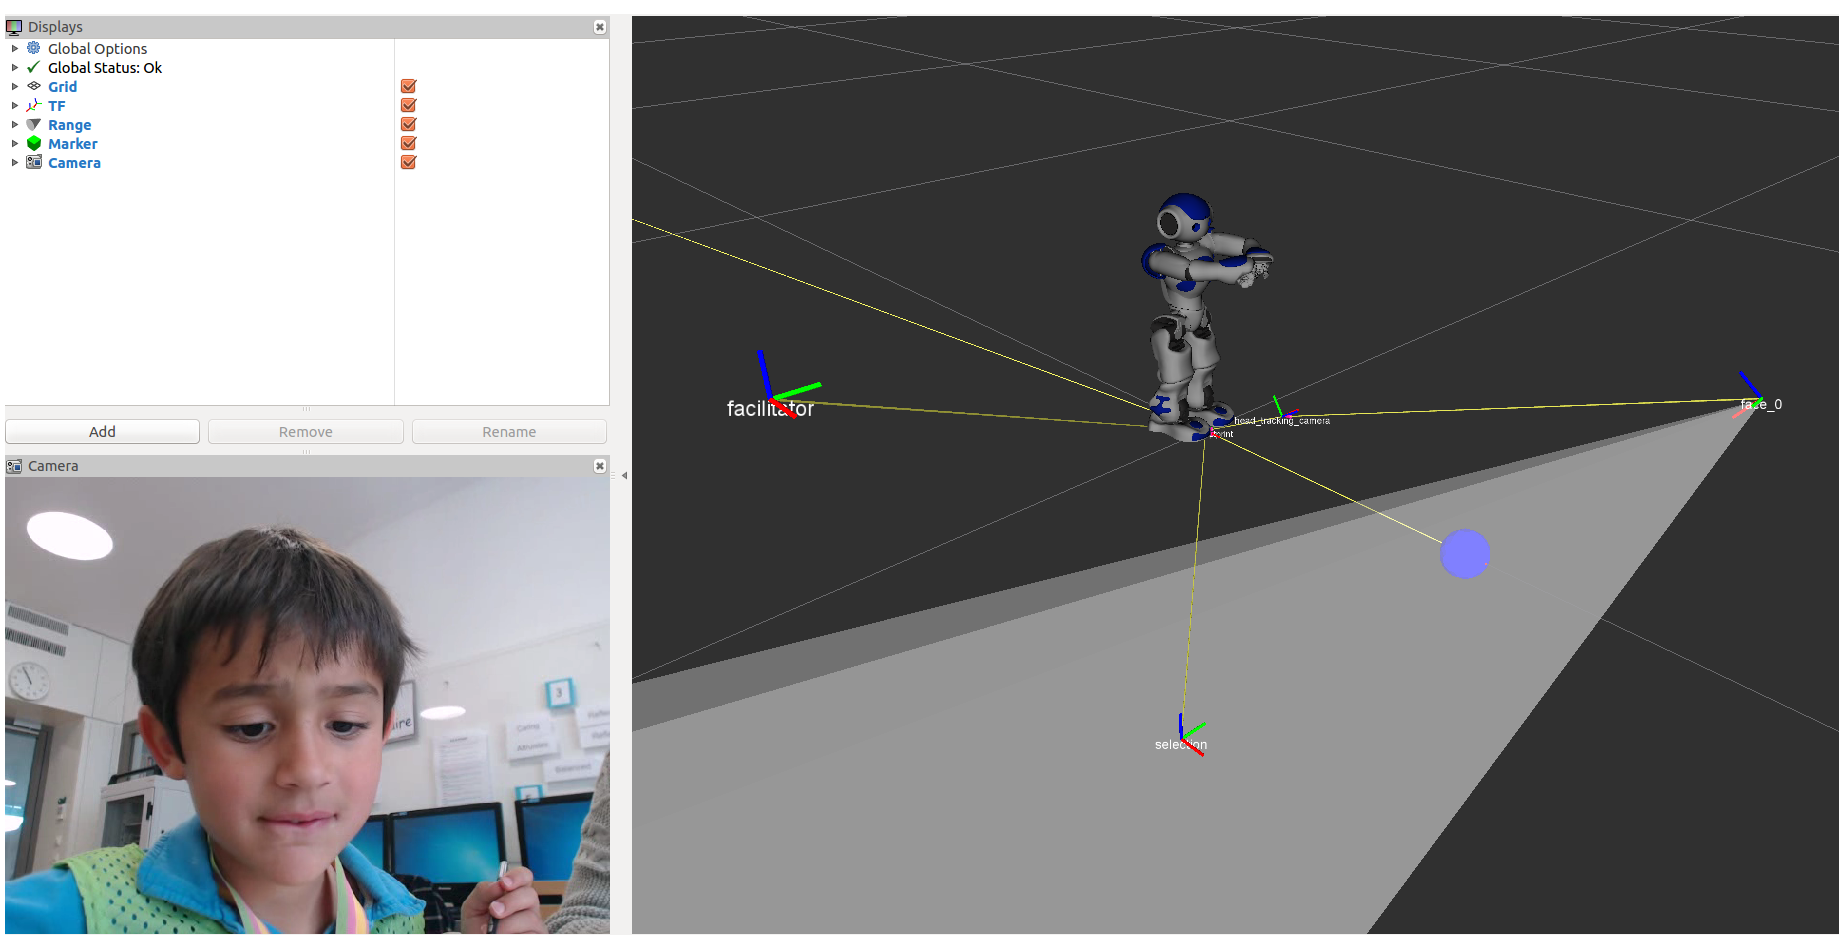
\includegraphics[width=1\columnwidth]{rviz}
    \caption{\small Rviz screenshot with Nao, camera (Nao's feet), face marker with VFOA (gray cone) and several static marker representations in the scene.}
    \label{rviz}
\end{figure}

\subsection{Estimating Head Pose}
The first step is to estimate the head pose using the pin-hole model shown in equation \ref{eq:pinHole}. As we mention before dlib library facilitates the task by providing the 2D points \textit{m'} that composes the face silhouette. However, it is enough with obtaining eight spread points, such as right and left eyes, right and left tragions, sellion or nasal depression zone, pronasale or center of the nose, stomion or center of the mouth and menton.

\newpage
Likewise, the 3D face model is needed. The proposed head pose estimation method would work best with a 3D face model of the query subject itself. When a 3D face model of the subject is not available, as in many practical situations, a 3D face model of a subject can be used. This is an estimation of the same anthropometric points \textit{M'} (for North American Caucasians) in the 3D space \cite{farkas1994anthropometry}. Moreover, the intrinsic camera parameters are necessary to be able to compose its matrix \textit{A}. The components are expanded in equation \ref{eq:pinHole2}.	

\begin{equation}
s  \; m' = A [R|t] M'
\label{eq:pinHole}
\end{equation}
\begin{equation}
s
\begin{bmatrix}
x \\
y \\
1
\end{bmatrix}
=
\begin{bmatrix}
f_x & 0 & c_x  \\
0 & f_y & c_y  \\
0 & 0 & 1 
\end{bmatrix}
\begin{bmatrix}
r_{11} & r_{12} & r_{13} & t_x  \\
r_{21} & r_{22} & r_{23} & t_y  \\
r_{31} & r_{32} & r_{33} & t_z  
\end{bmatrix}
\begin{bmatrix}
X \\
Y \\
Z \\
1
\end{bmatrix}
\label{eq:pinHole2}
\end{equation}

Finally, the matrix of extrinsic parameters [R|t] is obtained by joining the rotation matrix R (calculated from the rotation vector) and translation vector \textit{t}. The result is a matrix projection \textbf{P} which maps a point in the 3D space onto a point in the 2D image place solving the equation \ref{eq:p}.

\begin{equation}
s  \; m' = P \; M'
\label{eq:p}
\end{equation}

\subsection{Setting the \textit{tf} Frame}
The second step is to use the matrix [R|t] to set the correct translation and orientation of the \textit{tf} frame which represents the face in the 3D space. In order to achieve that it is necessary first, to set the origin defined by the vector \textit{t}. Second, the matrix \textit{R} needs to be reformulated into a quaternion as shown in equation \ref{eq:quat} due to the smoothly interpolation between them.

\begin{equation}
\begin{bmatrix}
qw \\
qx \\
qy \\
qz
\end{bmatrix}
=
\begin{bmatrix}
\sqrt{1 + r_{11} + r_{22} + r_{33}} /2 \\
(r_{32} - r_{23})/( 4 \cdot qw) \\
(r_{13} - r_{31})/( 4 \cdot qw) \\
(r_{21} - r_{12})/( 4 \cdot qw)
\end{bmatrix}
\label{eq:quat}
\end{equation}
\\
However, it is necessary to consider the cases where the division is performed by 0 (in 180\degree rotation about the y-axis for instance) or when \textit{qw} becomes close to zero.

\subsection{Defining the Field of View}
The third step is to generate a representation of the field of view which origin and orientation are the ones defined by the face detection \textit{tf} frame. 

Defining accurately the human field of view in the implementation is a must. Holmqvist in \cite{holmqvist2011eye} specifies that the visual human range is $ \pm  40\degree $ in the horizontal and $ \pm 25\degree $ in the vertical. In \cite{walker1980clinical} Spector provides a more detailed specification for each eye splitting the vertical range into $ 60\degree $ the upper region and $ 75\degree $ the lower one. Moreover, the horizontal range gets separated in $ 60\degree $ inwards (towards the nose) and $ 95\degree $ outwards. In the present implementation, the first approach explained has been chosen representing the field of view using a cone with such dimensions.

Assuming that the \textit{tf} frames representing the robotic agent, the two tablets, the experimenter and the observers are static, need to be monitored. This task consists on evaluating the intersection between the \textit{tf} frames and the field of view: If one focus of attention is within the region defined by the field of view, we assume the subject is looking at it. In order to solve such operation mathematically it is necessary to compute the transformation matrix between the coordinate frames to be able to locate the monitored frames \textit{A} in the subject's coordinate system \textit{B} (see equation \ref{eq:transform}).

\begin{equation}
v' = B(A^{-1})v
\label{eq:transform}
\end{equation}

where \textit{v} is a point in \textit{A} that becomes v' in coordinate system \textit{B}. However, in practice there are, at least, three different \textit{tf} frames involved in the transformation (subject-camera, camera-base, base-focus). Following the transformation result, the distance of the monitored frame with respect to the x-axis face \textit{tf} frame, $ d_{x_{axis}} $, representing the subject's face can be computed as simple as in equation \ref{eq:pitagoras}. Always considering the x-axis as the one defining the face's orientation and thus field of view's main axis.

\begin{equation}
d_{x_{axis}} = \sqrt{t_y^2 + t_z^2}
\label{eq:pitagoras}
\end{equation}

It is necessary to compare the distance acquired $ d_{x_{axis}} $ with the radius of the field of view at the target \textit{tf} frame x-coordinate $ r_{fov} $ as shown in equation \ref{eq:fovtf}.

\begin{equation}
r_{fov} = tan\left(\frac{fov}{2}\right) \cdot t_x
\label{eq:fovtf}
\end{equation}

where \textit{fov} is the aperture angle of the field of view. Finally, if $ d_{x_{axis}}<r_{fov} $, the target is within the subject's field of view.


% Plot to clarify this?

\section{Methodology}
\subsection{Experimental Set-up}

The target of this study were 6 children with ages compressed between 5 and 6 years old. The experiments were developed individually and consisted on a writing activity by turns and one story telling performed by the robot at a given time of the interaction. All this performed in a over all 20 minutes interaction average time.

Figure~\ref{realSetup} illustrates our general experimental setup: a
face-to-face child-robot interaction with an (autonomous) Aldebran's {\sc nao}
robot.

\begin{figure}
    \centering
    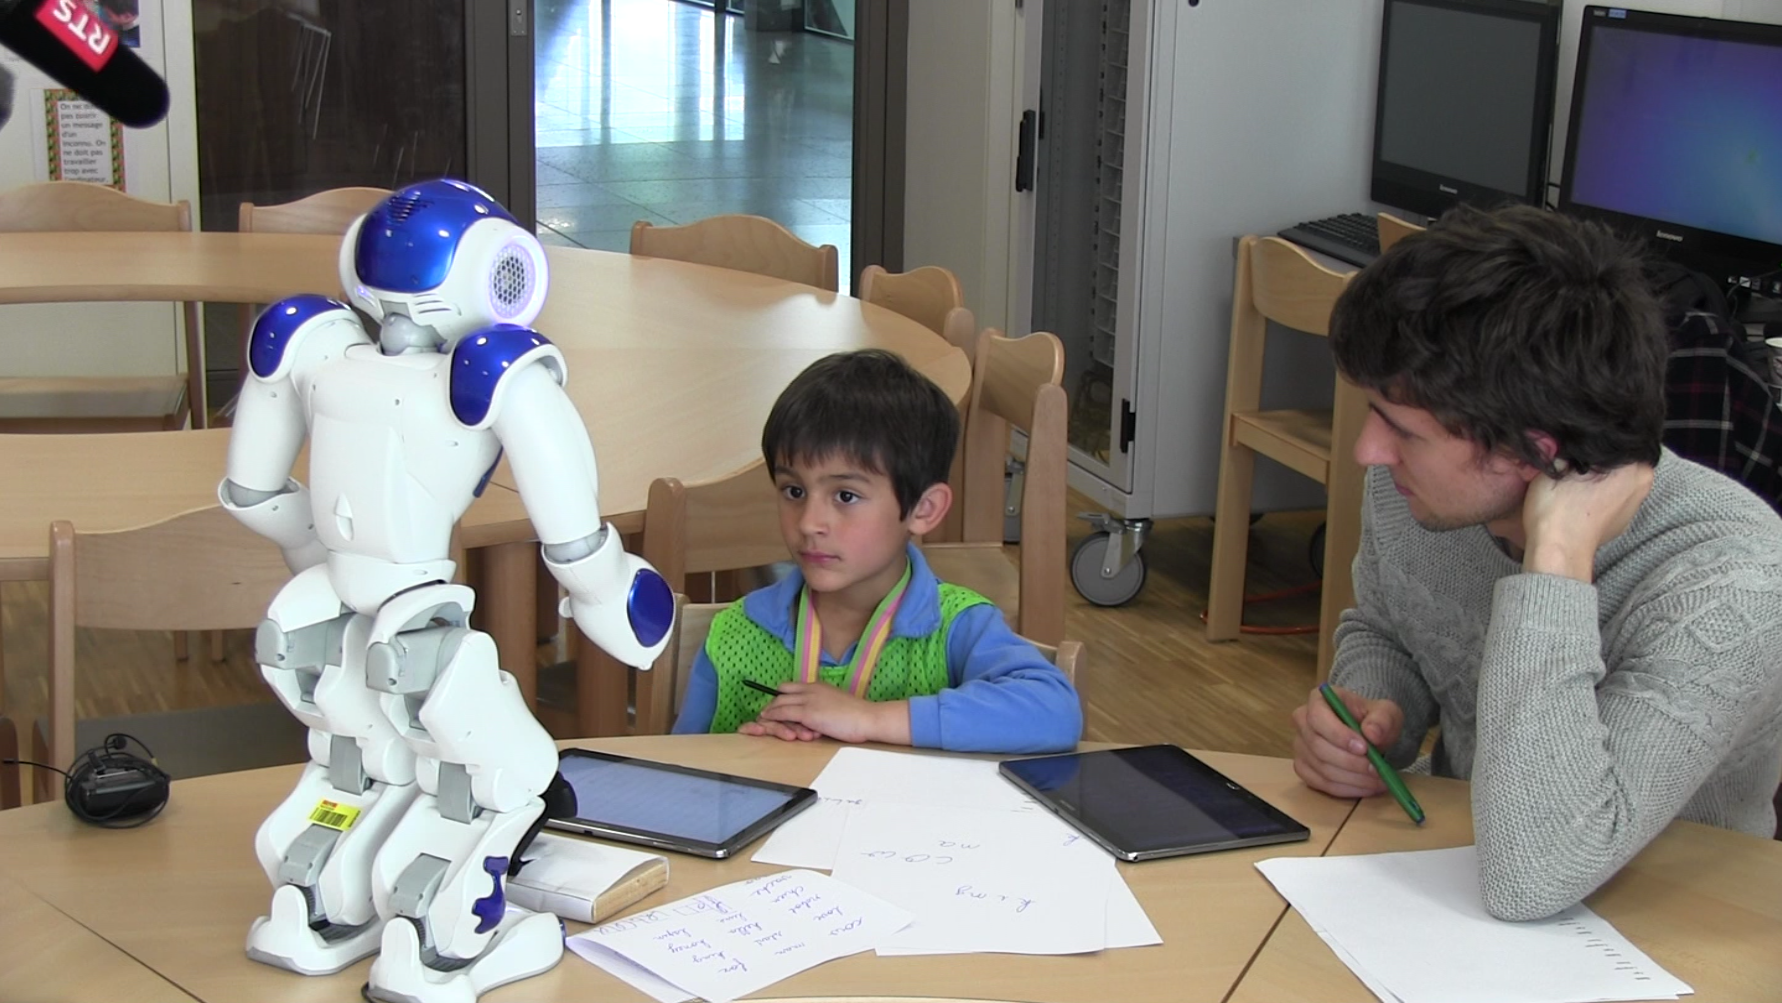
\includegraphics[width=1\columnwidth]{realSetup}
    \caption{\small Our experimental setup: face-to-face interaction with a {\sc
            nao} robot.  The robot writes on the tactile tablet, the child then
            corrects the robot by directly overwriting its letters on the tablet
            with a stylus. An adult (either a therapist or an experimenter,
            depending on the studies), remains next to the child to guide the work. 
            A second tablet allows to choose words and the camera captures the subject's face.}
    \label{realSetup}
\end{figure}

A tactile tablet (with a custom application) is used for both the robot and the
child to write: during a typical round, the child requests the robot to write
something (a single letter, a number or a full word), and push the tablet
towards the robot, the robot writes on the tablet by gesturing the writing (but
without actually physically touching the tablet), the child then pull back the
tablet, corrects the robot's attempt by writing him/herself on top or next to
the robot's writing (see Figure~\ref{fig:diego}), and ``send'' his/her
demonstration to the robot by pressing a small button on the tablet. The robot
``learns'' from this demonstration and tries again.

Since the child is assumed to take on the role of the teacher, we had to ensure
(s)he would be able to manage by him/herself the turn-taking and the overall
progression of the activity (moving to the next letter or word). In our design,
the turn-taking relies on the robot prompting for feedback once it is done with
its writing (simple sentences like ``What do you think?''), and pressing on a
small robot icon on the tablet once the child has finished correcting. In our
experiments, both were easy to grasp for children.

Implementing such a system raises several challenges that are discussed in detail in \cite{Hood:2015}.

An RGB camera has been used to acquire images of 640x480 pixels at 25 fps. The camera was located at 5 cm from the center of Nao's feet and its holder was tied to a wood base for stability purposes. Thus, the camera's objective was 9 cm above and $ 40\degree $ inclination with respect to the surface of the table. 
The subjects were typically located 50 cm away from the robot with the first tablet in front and the second one 30 cm to the left of the first one. In the same way, the experimenter was located around 60 cm to the left of the subject. Finally, two observers were located far away from the interaction field to manually assess the state of the interaction.

Figure \ref{drawSetup} allows us to intuitively identify several focuses of attention along the interaction such as the two tablets, the robot, the experimenter and the observers located in the diagonal.

\begin{figure}
    \centering
    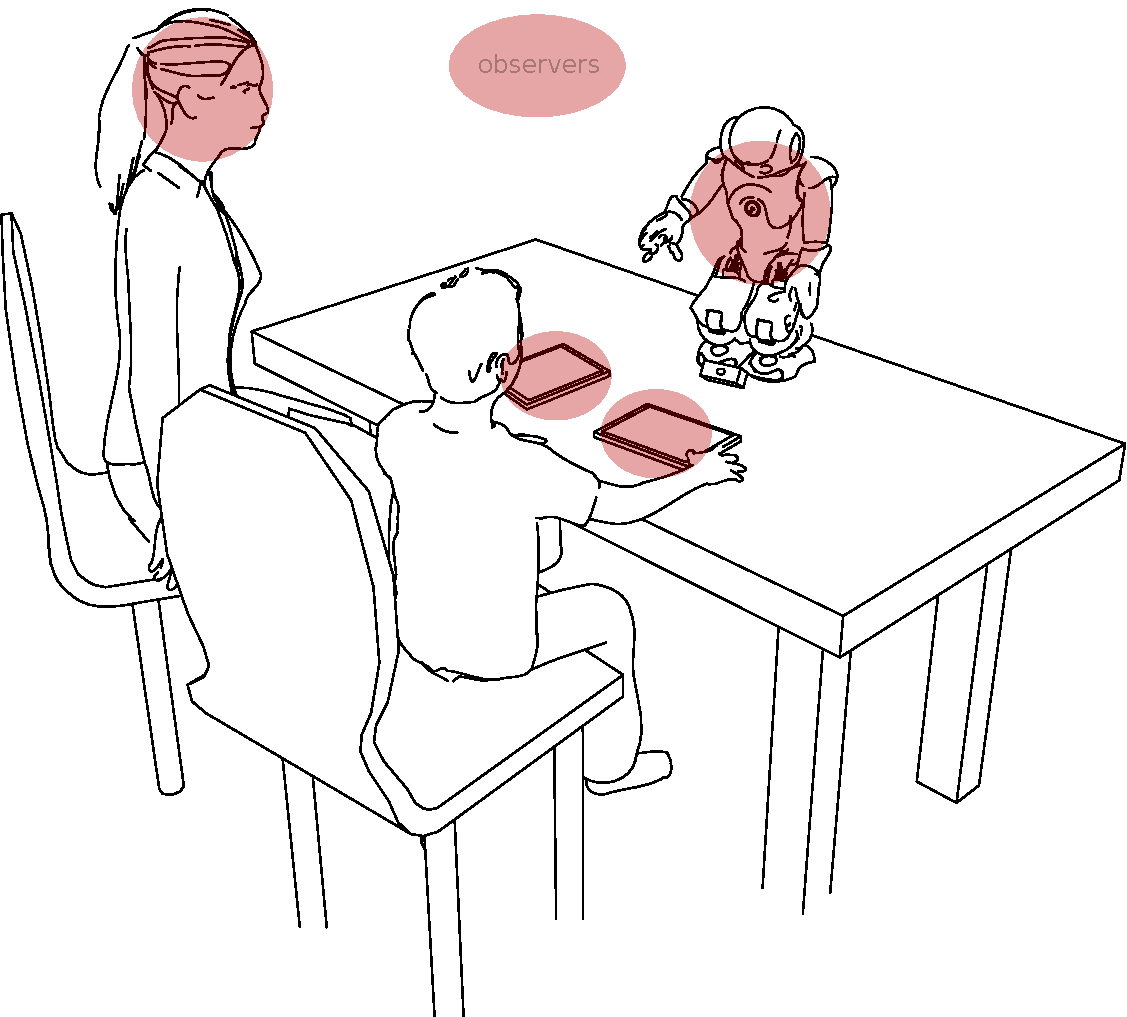
\includegraphics[width=0.7\columnwidth]{drawSetup}
    \caption{\small Graphical representation of he set-up and the possible children focuses of attention in the scene, in red.}
    \label{drawSetup}
\end{figure}


\section{Results}

In this work, head orientation is used to predict a person's focus of attention in face-to-face interactions. Therefore, we assume that head pose is a reliable marker of the attention focus during a social interaction, in both cases human-human, human-robot. Since we estimate where the subject is looking at based on its head position, several important questions arise:

\begin{enumerate}
\item Which head pose estimation tracking rate can we achieve during a real case scenario?  
\item How accurate can we predict where the subject is looking at based on the head pose estimation?
\item How can we evaluate the performance of the children based on the focus of attention?
\end{enumerate}

% Stats from the paper
% Stats from me
% Real vs captured plot
% Real vs expected plot

\subsection{From Face Detection to Focus of Attention}

According to \cite{stiefelhagen2002tracking} the head orientation's contribution in overall gaze direction is 68.9\% showing agreement between both measurements. In addition, it shows that the head orientation alone can get an average accuracy of 88.7\% detecting the focus of attention in a meeting application scenario using a head-mounted display with eye and head tracking.

Our results for a peer-to-peer work scenarios using an approach based on RGB camera are summarized in table \ref{tab:results} where the \textit{expected} is the focus of attention that given the state of the system, it is likely to attract the subject's gaze. In the same manner, the \textit{captured} is the focus of attention our approach provides and the \textit{real}, the ground truth of the subject's gaze direction based on manual annotations from two evaluators with an average reliability of $ \alpha--------\% $.

In order to calculate the inter-rater reliability between the two measurements (real-captured and real-expected), the overlap percentage between the two curves has been computed. A more reliable measurement between the real and captured focuses of attention is provided using the cosine similarity. These results are shown in table \ref{tab:results}. 

\begin{table}[h!]
	\centering
	\caption{Tracking accuracy in face-to-face scenario}
	\begin{tabular}{|c|c|c|c|c|c|c|c|} \hline
	\small Subject & 1 & 2 & 3 & 4 & 5 & 6 & Avg\\ \hline
	\small Track(\%) & \small78.7 & \small81.1 & \small73.7 & \small75.6 & \small77.1 & \small68.7 & \small75.8 \\ \hline
	\begin{tabular}{@{}c@{}}\small Real vs \\ \small expected(\%)\end{tabular} & \small93.1 & \small  & \small & \small & \small & \small & \small \\ \hline
	\begin{tabular}{@{}c@{}}\small Real vs \\ \small captured(\%)\end{tabular} & \small59.4 & \small & \small & \small & \small & \small & \small \\ \hline
	\begin{tabular}{@{}c@{}}\small Cosine \\ \small affinity \end{tabular} & \small0.72 & \small & \small & \small & \small & \small & \small \\ \hline
	\end{tabular}
	\label{tab:results}
\end{table}

The results has shown that the percentage of accuracy in the tracking is not only conditioned by the subject's amount of movement, but also by the speed of the same movements: Restless children externalize greater levels of movement decreasing the tracker accuracy. Additionally, several recurrent computer vision challenges such as the lighting conditions, occlusions and the face angle with respect to the camera are factors that contribute to reduce the accuracy.

\subsection{Subject's Focus of Attention Analysis}


\begin{figure*}
    \centering
    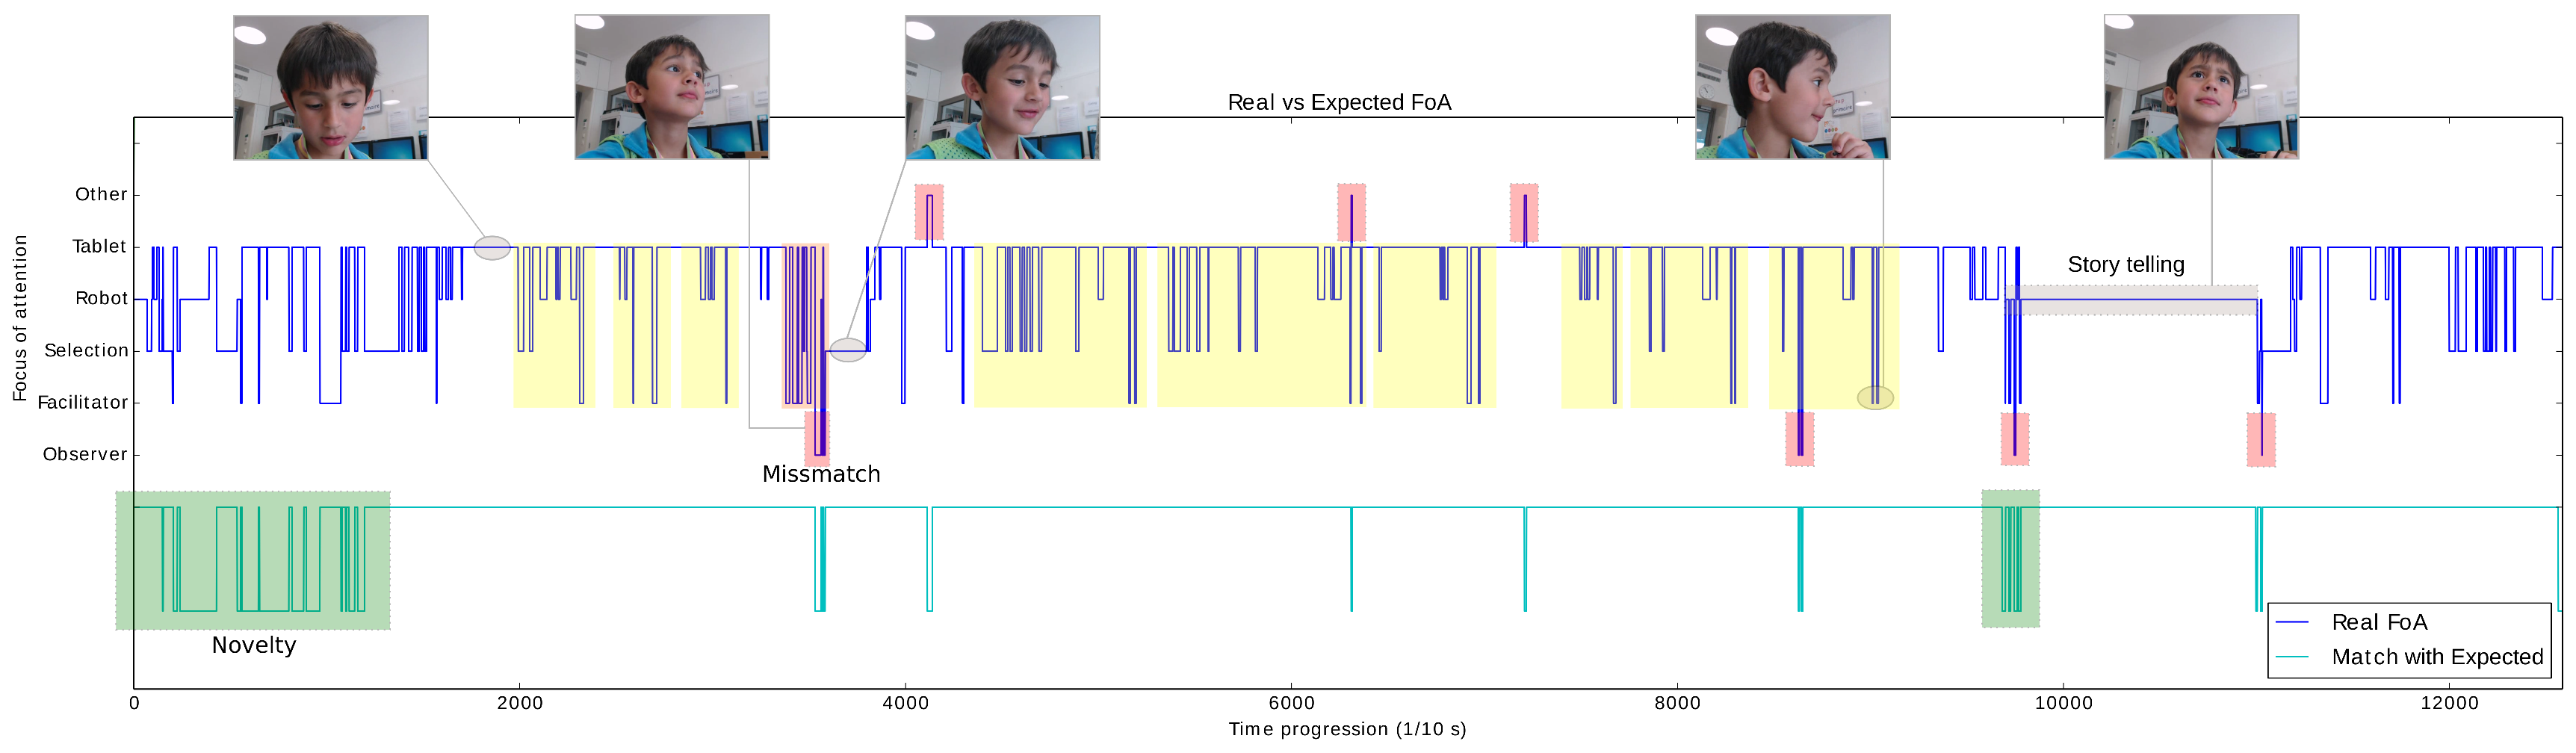
\includegraphics[width=2\columnwidth]{realExpected}
    \caption{\small In blue, real focus accoding to two observer assessment. In cyan, the overlap between the real and the expected focus of attentions. In yellow, the repeated pattern in turn-taking and orange is the experimenter's suggestion to switch to a difficult word}
    \label{fig:realExpected}
\end{figure*}


\begin{figure*}
    \centering
    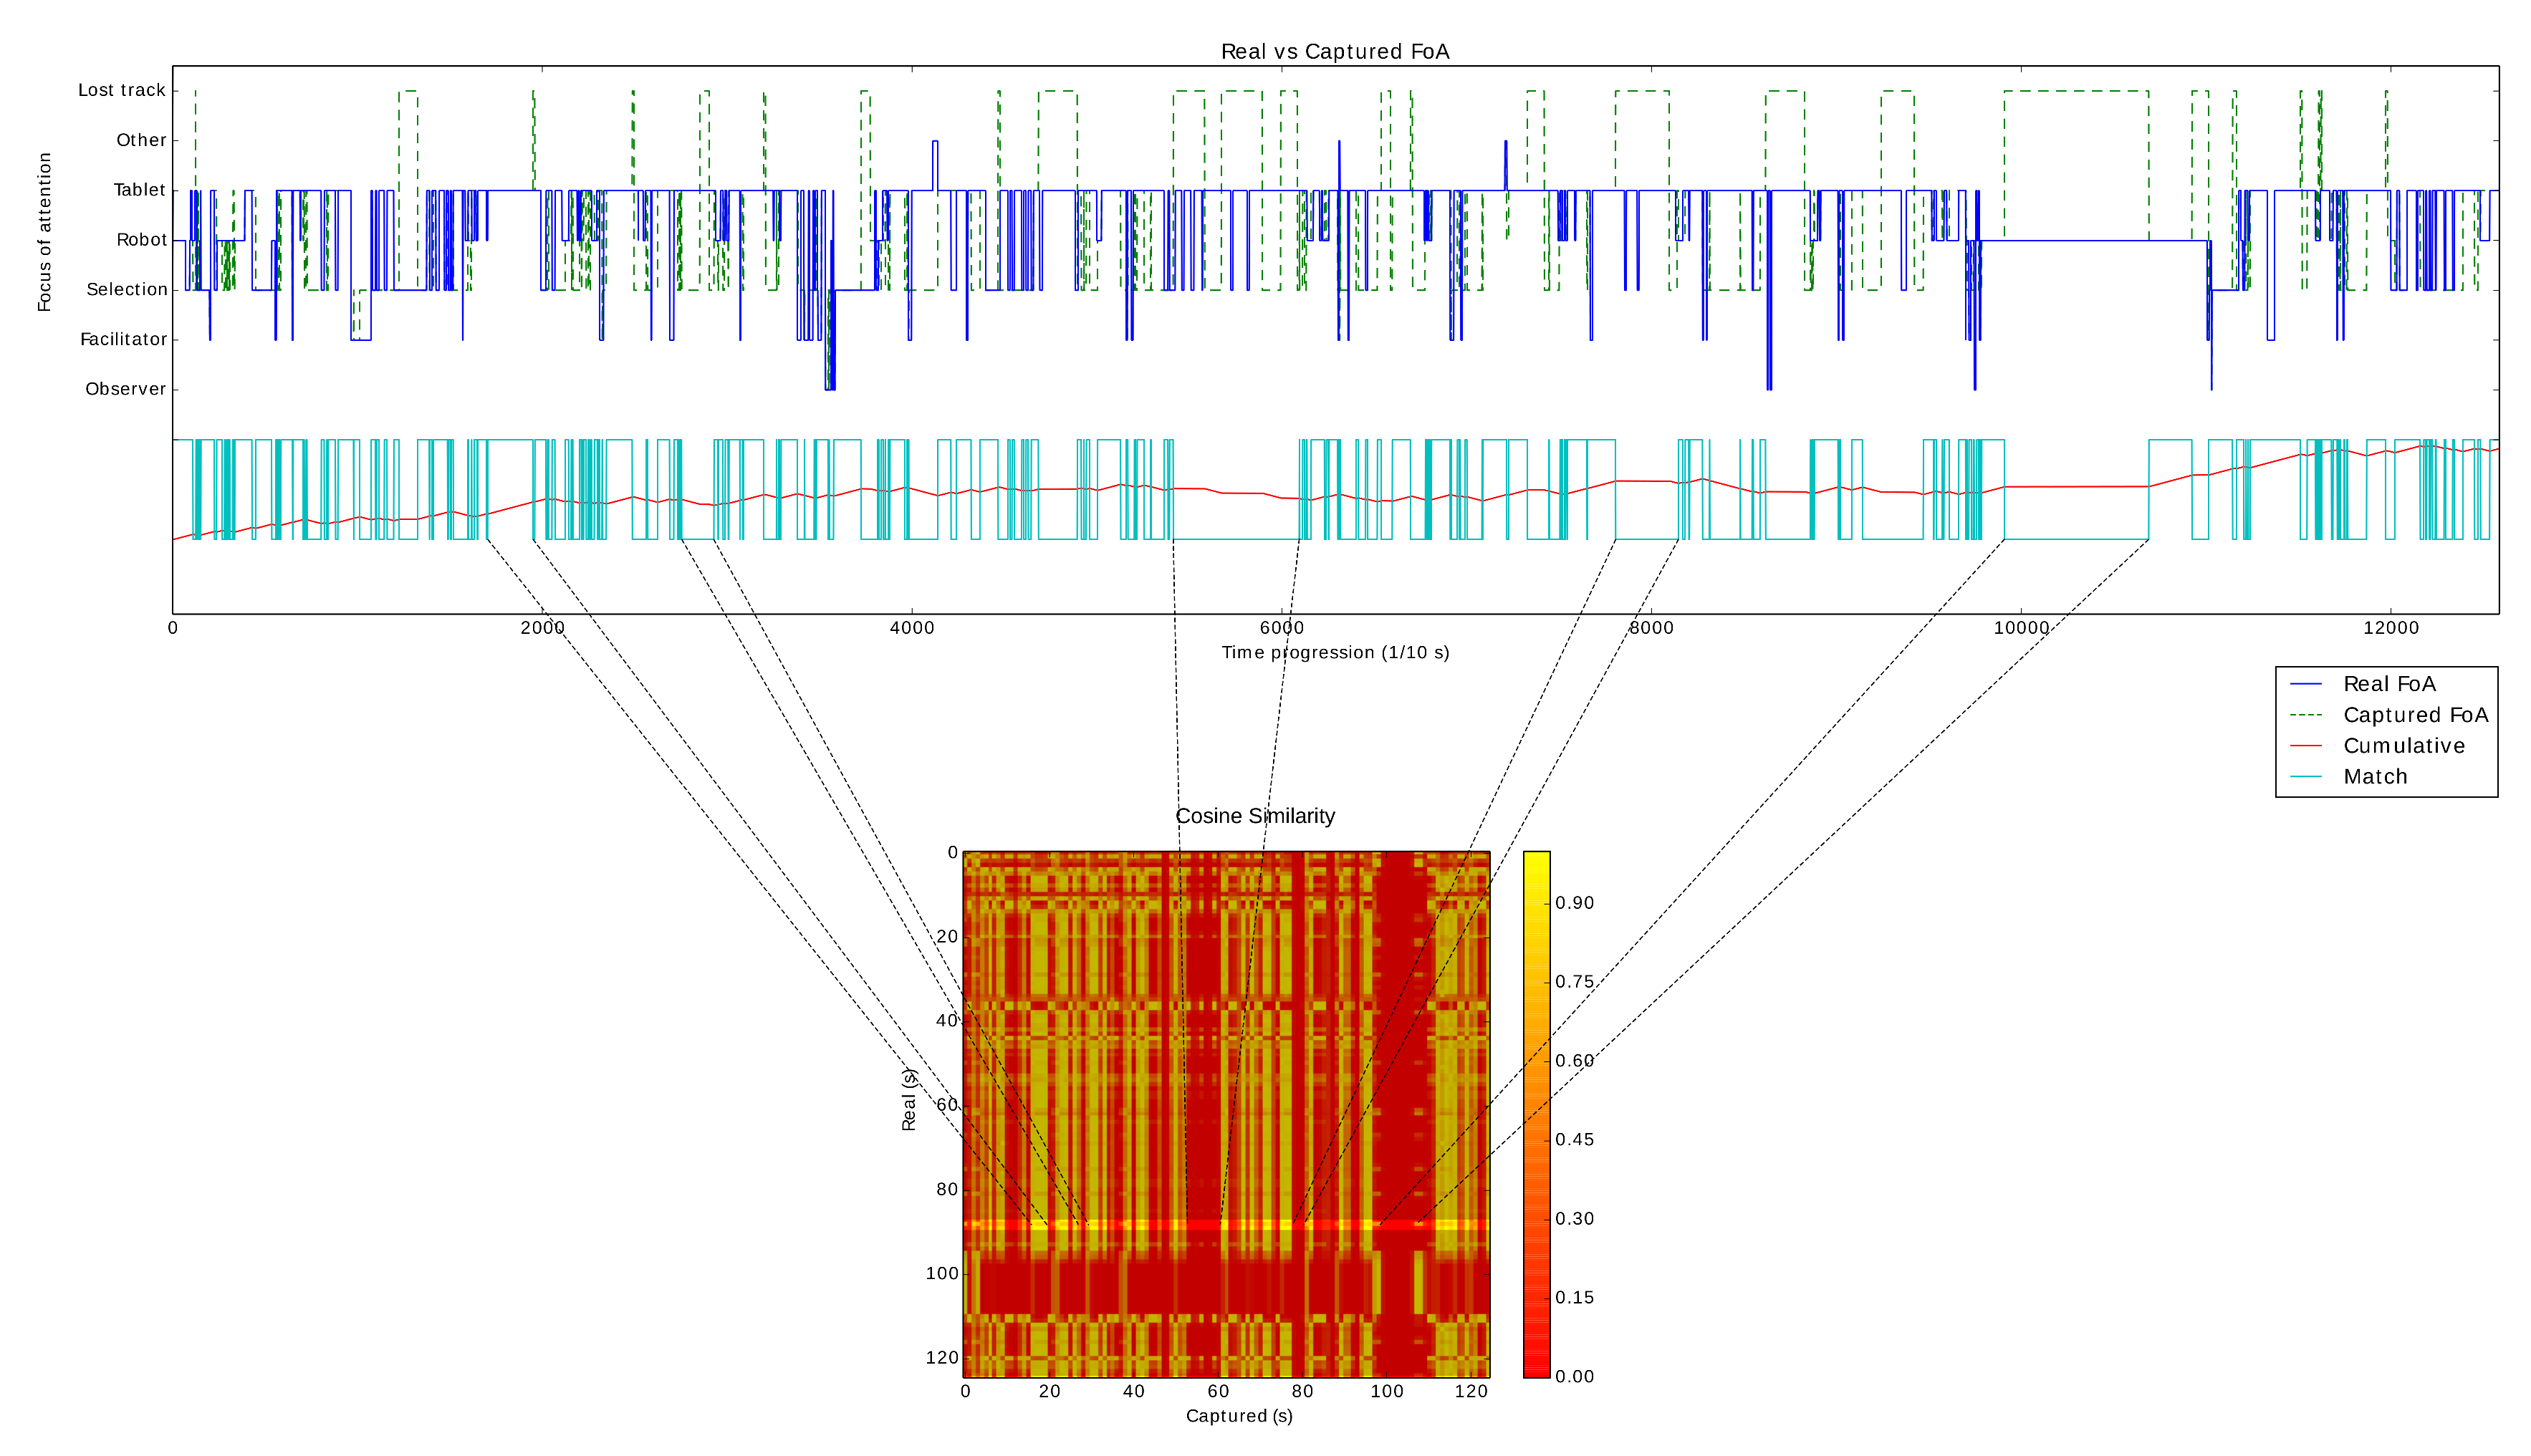
\includegraphics[width=2\columnwidth]{bitmap_zoom}
    \caption{\small At the top in blue, the real focus accoding to two observer assessment. In green, the captured focus using our aproach and in cyan, the overlap between them. At the bottom, the cosine similarity matrix between both curves with a window size of 10 seconds.}
    \label{fig:realCaptured}
\end{figure*}


In several occasions during the interaction, none of the focuses of attention were within the field of view due to the time transition from one focus to another. In order to deal with these few cases we assume that the minimum distance between the height of the field of view (cone) and the targets corresponds to the most likely focus of attention.

However, we also want to distinguish such cases when the subject is directly not looking where the defined targets are located, but towards a region far from the interaction field. These cases are not common but they can be easily identified by setting a horizontal threshold to the field of view.

Several results can extracted from figure \ref{fig:realExpected}. First, the matching curve shows the overlapping between the expected and the real focuses of attention. As we can see there is a fluctuation at the beginning of the interaction suggesting a novelty effect. It suggests that the adaptation time is around the first 2 minutes in average. 

Second, once the turn-taking is established, a pattern becomes visible during the subject's feedback, when a word is being written by the children: Such pattern shows a high intermittent gaze frequency from the tablet to the selection. It shows that the subject is using the word model in the selection tablet to provide a better answer to the robot. But not only that, the subjects also decrease the response time after each shift as well as the gaze frequency towards the model suggesting and improvement over time. Moreover, when a new word is selected for playing, the same behavior is replicated (see yellow boxes in figure \ref{fig:realExpected}).

A third trend that can be observed is the continuous 'look for approval' situation where the subjects look at the experimenter in order to provide feedback about the robot's response before providing their own one (see yellow boxes in figure \ref{fig:realExpected}). Such transition tablet-experimenter becomes more frequent in several cases, for instance: An unexpected situation is faced (before the story telling) or the experimenter makes a suggestion (orange box in figure \ref{fig:realExpected}).

Finally, the subjects set their attention more often to the tablet displaying the generated hand-writing during the robot feedback rather than to the robot itself. 


%what do you think? -> tablet -> robot -> facilitator -> pattern

%Too much gaze to selection: the challenge may be too big, let's adapt response from robot

%Use time to account quality of interaction?

\section{Conclusions}
The rate of attention shift can predict retained learning.
%Support this with a plot averaging all interactions of all subjects 
The solution presented can be adapted to work in new locations
Thanks to their easiness of use in real world scenario, due to employment of non-intrusive sensors



%. Less time means better understanding a move to next level.
%Future work
Possible focuses of attention has to be known in advance.  
Our system could be extended to allow both user and robot to move freely.
develop the concept of gaze-aware robot Woud be nice to do it in an unconstrained environment.

It is necessary to take into account that eye gaze information is neglected which induces a certain amount of error, as well as the noise induced by the 3D pose estimation computed from face landmarkers.

From first person videos -> we put the camera there to maximize the detection during the writing time but it could installed in the head of the robot as tf even with movement constantly updating the tf frame matrix.


%ACKNOWLEDGMENTS are optional
\section*{Acknowledgments}
This research was partially supported by the Funda\c{c}\~{a}o para a Ci\^{e}ncia
e a Tecnologia (FCT) with reference UID/CEC/ 50021/2013, and by the Swiss
National Science Foundation through the National Centre of Competence in
Research Robotics.

\bibliographystyle{abbrv}
\bibliography{sigproc}
\end{document}
